%% BEGIN semsamp2.tex
% This is a sample document for seminar.sty, v0.93 (and maybe later).
%
% This file contains both landscape and portrait mode slides.
% Choose one of the following to print them out:
%  - If using PSTricks, try the semcolor style option.
%  - If using Rokicki's dvips, try the semrot style option.
%  - To print the landscape slides, put \landscapeonly in the preamble.
%    To print the portrait slides, include the portrait style option and
%    put \portraitonly in the preamble.
%
%
\documentclass[%
%rrrrrrrrrrrrrrrr\documentstyle[%
  slidesonly,%  Try notes or notesonly instead.
  %10pt,%notes,%      Use instead of slidesonly to typeset the notes.
  %notesonly,%  Use instead of slidesonly to typeset notes and slides.
  %semcolor,%   Try me if using PSTricks.
  %semrot,%     Try me if using Rokicki's dvips.
  %semhelv,%    Try me if using a PostScript printer.
  %article,%    Try me.
  %portrait,%   Try me.
  %sem-a4,%     Try me if using A4 paper.
  semlayer%     This must be included, but you need the semcolor option to
  ]{seminar}                                  % actually see the overlays.

\slidesmag{5}
\articlemag{1}

%\twoup                     % Try me for twoup printing.

%\portraitonly              % To print only portrait slides
%\landscapeonly             % To print only landscape slides

%\notslides{\ref{questions}-7,1}   %Try me: The slides are omitted.
%\onlyslides{\ref{questions}-7,1}  %Try me: Only these slides are included.
%\onlynotestoo                     %Try me: For selecting notes as well.

\colorlayers{red,blue}      % Try deleting this if using the semcolor option,
                            % to get \blue and \red to use PostScript color.

%\overlaysfalse             % Suppress overlays with semcolor option.
%\layersfalse               % Suppress color layers with semcolor option.

\rotateheaderstrue          % Try this out if using rotation macros.

\usepackage{hyperref}
\usepackage{url}
\usepackage{amsmath}
\usepackage{amsthm}
\usepackage{graphicx}
% \usepackage[pdftex]{graphicx}
\usepackage{amsfonts}
\usepackage{mathrsfs}
\usepackage{amssymb}
\usepackage[noend]{algorithmic}
\usepackage[plain]{algorithm}
\usepackage{subfigure}

\usepackage{color}
\usepackage{ulem}

%\newtheorem{theorem}{Theorem}[section]
\newtheorem{theorem}{Theorem}
\newtheorem{corollary}{Corollary}[section]
\newtheorem{lemma}{Lemma}[section]
\newtheorem{definition}{Definition}[section]
\newtheorem{proposition}{Proposition}[section]
\newtheorem{claim}{Claim}[section]
\newtheorem{model}{Model}[section]
\newtheorem{example}{Example}[section]
%\newtheorem{algorithm}{Algorithm}[section]
%\newenvironment{proof}{\noindent{\bf Proof.}}{\hspace*{\fill} $\Box$}
%\newenvironment{defn}{\noindent \underline{\hspace{7in}}\\ \noindent{\bf Defn:}}{\hspace*{\fill} \newline\noindent\underline{\hspace{7in}}}
\newenvironment{defn}{\noindent \\ \noindent{\bf Defn:}}{\hspace*{\fill} \newline}
\newcommand{\fns}{\footnotesize}
\newcommand{\sk}{\sf{sk}}
\newcommand{\pk}{\sf{pk}}
\newenvironment{thm}{\noindent{\bf Theorem:}}{\hspace*{\fill} }
\newcommand{\bare}{\noindent \underline{\hspace{7in}}\\ }
%\newcommand{\myws}{\textcolor{white}{ XXXXXX}}
\newcommand{\vt}{

\vspace{.15in} 

\noindent}

\newcommand{\nvt}{

\vspace{-.15in} 

\noindent}
%\newenvironment{thm}{\noindent{\bf Theorem:}}{\hspace*{\fill} }
%\newcommand{\bare}{\noindent \underline{\hspace{7in}}\\ }
%\newcommand{\myws}{\textcolor{white}{ XXXXXX}}
%\newcommand{\mybul}{{\textcolor{white}{XX}}$\bullet$ }
\newcommand{\myar}{\textcolor{red}{ ==$>$}}
\newcommand{\mybl}{{\textcolor{white}{XX}}{\bf *}}
\newcommand{\n}{\noindent }

\newcommand{\mylg}{\mbox{ lg } }



\newcommand{\tht}{\hspace{.15in} }

\newcommand{\Half}{\mbox{\bf Half}}
\newcommand{\Solve}{\mbox{\bf Solve}}
\newcommand{\Halfc}{\underline{\mbox{\bf Half}}}
\def\4halftbs{XXX\=XXXX\=XXXX\=mmm\kill}

\def\tbs{XXXXXXX\=XXXXX\= \kill}
\def\otbs{XXXXXXX\=XXXXX\=XXX\=XXX\= \kill}
\def\sqrotbs{xxx\=xxx\=xx\kill}
\def\lsqrotbs{xxx\=xxx\=xxx\=xxBBBBBBBBBBBBBBBBBBBBBBBBBBBB\=xxx\=lxx\=xx\kill}
\def\monttbs{xx\=xxxx\=xxxx\=xxxx\kill}
\def\knudtbs{xxx\=xxxx\=xxxx\=xxxx\kill}

\renewcommand{\baselinestretch}{1}
\setlength{\unitlength}{.1in}
\addtolength{\textheight}{1.3in}
\addtolength{\topmargin}{-1.3in}
\addtolength{\textwidth}{1.88in}
\addtolength{\evensidemargin}{-1in}
\addtolength{\oddsidemargin}{-.9in}

\title{Chapter 1: Introduction}
\author{}
\date{}

\newcommand{\sref}[1]{SLIDE \ref{#1}}
\newcommand{\heading}[1]{\begin{center}\large\bf #1\end{center}}

\newpagestyle{MH}%
  {Purdue School of Eng \& Tech Graduate Student \LaTeX Workshop\hfil\thepage}{}
\pagestyle{MH}



%\begin{document}
\def\otbs{XXXXXXX\=XXXXX\=XXX\=XXX\= \kill}
\def\proofpartbs{XXX\=XXXXXxxxxxxxxxxxxxxxxxxx\=XXX\=XXX \kill}
\date{}
\newcommand{\ovec}{\overline}
\newcommand{\ds}{\displaystyle}
\newcommand{\ar}{\longrightarrow}
\newcommand{\p}{\prime}
\newcommand{\z}{{\bf Z}}
%\newcommand{\r}{{\bf R}}
\newcommand{\ex}{\noindent {\bf Example} }
\newcommand{\ra}{{\ Longrightarrow}}
\newcommand{\md}{{\makebox{ mod }}}
%\newcommand{\n}{{\noindent}}
\newcommand{\deriv}{\ds{\frac{dy}{dx}}}
\newcommand{\recipderiv}{\ds{\frac{dx}{dy}}}
\newcommand{\tab}{{\hspace{.3in}}}
\def\monttbs{xx\=xxxx\=xxxx\=xxxx\kill}
%\newcommand{\tht}{\hspace{.15in} }
\newcommand{\myws}{\textcolor{white}{XX}}
\newcommand{\mybul}{{\textcolor{white}{XX}}$\bullet$ }
\newcommand{\mystr}{{\textcolor{white}{XXXXXX}}$ \diamondsuit $ }
%\newcommand{\myar}{\textcolor{red}{ ==$>$}}
\newcommand{\la}{\longleftarrow}
\newcommand{\ty}{\textcolor{red}}
% Math-mode symbol & verbatim
\def\W#1#2{$#1{#2}$ &\tt\string#1\string{#2\string}}
\def\X#1{$#1$ &\tt\string#1}
\def\Y#1{$\big#1$ &\tt\string#1}
\def\Z#1{\tt\string#1}




%\pagestyle{empty}
\newcommand{\nhp}{\mbox{\it No half point}}
%\def\tbs{xxx\=95 - 100 $\%$\=xxxx\=95 - 100 $\%$\=xxxx\=95 - 100 $\%$
%\=xxxx\=95 - 100 $\%$\=xxxx\=95 - 100 $\%$\=xxxx\=mmm\kill}
\def\mtbs{xxxxxxx\=95 - 100 $\%$\=xxxx\= xxxxx\=\kill}
\def\smtbs{xxxxxxx\=95 - 100 $\%$xxxxxxxxxxxxxxx\= xxxxx\kill}
\def\sqrotbs{xxx\=xxx\=xx\kill}
%\def\lsqrotbs{xxx\=xxx\=xxx\=xxBBBBBBBBBBBBBBBBBBBBBBBBBBBB\=xxx\=lxx\=xx\kill}
\def\pkcset{\= $|E_{a_2,a_6}|=p\cdot 2$xxxx \= cofactor $2$xxx \=  $|(x,y)|=2n$ bitsxxxx \= compressed to $n$\kill}


%\def\lsqrotbs{xxx\=xxx\=xxBBBBBBBBBBBBBBBBBBBBBBBBBBBB\=xxx\=lxx\=xx\kill}

%.b.b.b.b.\def\lsqrotbs{xxx\=xxx\=xxx\=xxBBBBBBBBBBBBBBBBBBBBBBBBBBBB\=xxx\=lxx\=xx\kill}
\def\lsqrotbs{xxx\=xxx\=xxx\=xxBBBBBBBBBBBBBBBBBBBBBBBBBBBB\=xxx\=xxx\=lxx\=xx\kill}


% *********************************************************************************
% *****************************************************************
\newcommand{\mfor}{{\bf for }}
\newcommand{\mdo}{{\bf do }}
\newcommand{\melse}{{\bf else }}

\newcommand{\mif}{{\bf if }}
\newcommand{\mthen}{{\bf then }}
\newcommand{\mwhile}{{\bf while }}
\newcommand{\htab}{\tab}

\newcommand{\vtab}{{

\vspace{.2in} 

\n}}
\begin{document}
\DeclareGraphicsExtensions{.pdf, .bmp,.png,.gif,.jpg}


\maketitle          % This won't show up when \onlynotestoo is in effect.

\begin{slide}
  \ifslidesonly              % Title slide only for slidesonly selection.
    %\maketitle
    \addtocounter{slide}{-1}
    \slidepagestyle{empty}
  \fi
\end{slide}


\begin{slide}

\footnotesize

\begin{center}
\section*{Secure Data Aggregation Protocol for Sensor Networks}
  \vfill
  Presented By : Kavit Shah

  Major Advisor : Brian King
  
  Thesis Committee Members : Paul Salama, Mohamed El-Sharkawy, Sangkook Lee
  \vfill
  \end{center}
  \clearpage

\section*{Overview}
  \vfill
  \begin{center}
    \begin{itemize}
      \item Introduction
      \item Data Aggregation
      \item Secure Hierarchical In-network Data Aggregation (SHIA)
      \item Our Protocol
      \item Conclusion
    \end{itemize}
  \end{center}
  \vfill
  \clearpage

\section*{Introduction}
  \vfill
  \begin{description}
    \item[Ubiquitous Computing -] is a scenario in which computing is everywhere.

    \item[Internet of Things -] is a system where the Internet is connected to physical world via ubiquitous sensors.
    
    \item[Ad-hoc Networking -] is a local network of sensors formed by peer-to-peer communications.
    
    \item[Sensor Networks -] Collectively, we refer these concept as Sensor Networks.
  \end{description}
  \vfill
  \clearpage

  \subsection*{Sensor Networks}
    \vfill  
    In sensor networks, thousands of sensors may interact with each other and collects raw data.

    The data is processed by computationally powerful machine (the base station).

    Then the base station converts data into information.

    Based on the information an important action is taken.

    % \begin{figure}[h!]
    %   \centering
    %   % \includegraphics{images/swon.pdf}
    %   % 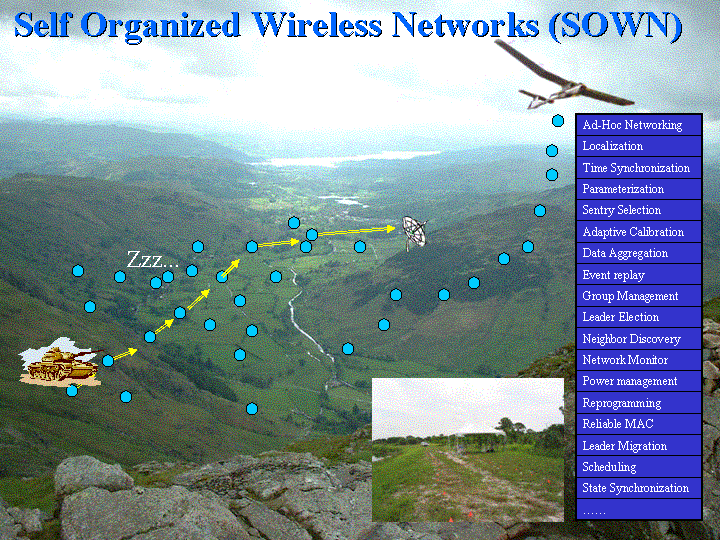
\includegraphics{swon.png}
    %   \caption{Sensor Network}
    %   \label{fig:sensor-network}
    % \end{figure}
    \vfill
    \clearpage

  \subsection*{Sensor Networks Applications}
    \vfill
    \begin{description}
    \item[Military -] enemy tracking, battle filed surveillance or target classification.

    \item[Environmental -] to monitor geographical location without much human intervention.
    
    \item[Health Care -]  to monitor patients around the clock, send reminders to doctors and nurses.
  
    \item[Sustainable Mobility -] to build digitally connected and coordinated vehicles.
    \end{description}
    \vfill
    \clearpage

  \subsection*{Consequences of Sensor Failures}
      \vfill
      Speed sensor failure led to crash of Air France flight - Airbus A$330$-$203$ AF $447$ on $1$st June $2009$.
      
      \textbf{For nearly a minute}, as the speed sensors jumped, the pilot was not present in the cockpit. 

      The pilots could not reclaim control as the plane dropped out of the sky at a rate of \textbf{10,000 feet per minute}.
          
      The flight plunged into the Atlantic nose-up after its three-and-a-half minute freefall , killing all \textbf{228} on board.      
      \vfill
      \clearpage

  \subsection*{Resource Constrains in Sensor Network}
    \vfill
    \begin{description}
      \item[Physical Limitations -] often deployed in open, hostile and unattended environments.

      \item[Hardware Limitations -] due to lower manufacturing cost of sensor nodes, they have low speed processor, limited storage, a short range trans receivers.

      \item[Transmission Medium -] wireless networks have approximately \textbf{$10^6$ times higher bit error rate (BER)} than wired networks which causes frequent link loss and then path loss.

      \item[Mobility -] network topology is dynamic, topology changes due to link failure, node failure or bandwidth optimization.
    \end{description}
    \vfill
    \clearpage

\section*{Cryptographic Tools}
  \vfill
  \subsection*{Hash Functions}
    A hash function takes a message as its input and outputs a fixed length message called hash code, creating a digital fingerprint of the message.

    % A hash function $h$ should have the following properties :
    \begin{description}
      \item [Compression] A function $h$ maps an input $x$ of arbitrary finite bitlength, to an output $h(x)$ of fixed bitlength $n$.
      \item [Preimage resistance] For all pre-specified outputs, it is computationally infeasible to find any input which hashes to that output, i.e., to find any preimage $x'$ such that $h(x') = y$ where $y$ is given whose corresponding input is not known.
      \item [2nd-preimage resistance] It is computationally infeasible to find any second input which has the same output as any specified input, i.e, given $x$, to find a 2nd-preimage $x' \neq x$ such that $h(x') = h(x)$.
      \item [Collision resistance] It is computationally to find any two distinct inputs $x,x'$ which hash to the same output, i.e., such that $h(x) = h(x')$.
    \end{description}
    SHA-256, is a 256-bit hash and provides $128$ bits of security against collision attacks.
    \vfill
    \clearpage

  \subsection*{Message Authentication Codes}
    \vfill
    A Message Authentication Code (MAC) is a family of hash functions parameterized by a secret key $k$.

    \begin{description}
      \item [Ease of computation] For a known function $h_{k}$, given a value $k$
      and an input $x$, $h_{k}(x)$ is easy to compute.
      \item [Compression] A function $h_{k}$ maps an input $x$ of arbitrary finite bitlength to an output $h_{k}(x)$ of fixed length $n$.  
      \item [Computation-resistance] Given a description of the function family $h$, for every fixed allowable value of $k$ (unknown to an adversary), given zero or more text-MAC pairs ($x_{i}, h_{k}(x_{i})$), it is computationally infeasible to compute any text-MAC pair ($x,h_{k}(x)$) for any new input $x \neq x^{'}$ (including possibly for $h_{k}(x) = h_{k}(x_{i})$ for some $i$). 
      If computation-resistance does not hold, a MAC algorithm is subject to MAC-forgery.
    \end{description}
    \vfill
    \clearpage

  \subsection*{Digital Signatures}
    \vfill
    A digital signature is a cryptographic scheme for demonstrating the authenticity of a digital message.
    
    A valid digital signature gives a recipient strong reason to believe that the message was created by a known sender, such that the sender can not deny having sent the message (\textbf{authentication and non-repudiation}) and that the message was not altered in transit (\textbf{integrity}).

    It is a 5-tuple scheme ($\mathcal{M}$, $\mathcal{K}$, $\mathcal{G}$, $\mathcal{S}$, $\mathcal{V}$)

    % \begin{enumerate}
    %   \item a plain text message space $\mathcal{M}$ (set of strings over alphabets)
    %   \item a signature space $\mathcal{S}$ (set of possible signatures)
    %   \item a signing key space $\mathcal{K}$ (set of possible keys for signature generation) and a verification space $\mathcal{K^{'}}$ (a set of possible verification keys)
    %   \item an efficient key generation algorithm \textsf{Gen} : $N \rightarrow$ $\mathcal{K} \times \mathcal{K^{'}} $ 
    %   \item an efficient signing algorithm \textsf{Sign} : $ \mathcal{M} \times \mathcal{K} \rightarrow \mathcal{S}$
    %   \item an efficient verification algorithm \textsf{Verify} : $\mathcal{S} \times \mathcal{M} \rightarrow$ \{true, false\} 
    % \end{enumerate}
    For any secret key $s_{k} \in \mathcal{K}$ and any $m \in \mathcal{M}$, the message $m$ is signed using key $s_{k}$ as follows:
      \begin{equation}
        s = \textsf{Sign}_{s_{k}}(m)
        \label{eq:signature}
      \end{equation}
    For any $s_{k}$ let $p_{k}$ denote public key and for all $m \in \mathcal{M}$ and $s \in \mathcal{S}$, $s$ as follows:
    \begin{equation}
      \textsf{Verify}_{p_{k}}(m,s) = 
      \begin{cases}
       \textbf{true}\ \mbox{with probability of 1} & \mbox{if}\ s = \textsf{Sign}_{s_{k}}(m)\\
       \textbf{false}\ \mbox{with overwhelming probability} & \mbox{if}\ s \neq \textsf{Sign}_{s_{k}}(m)
      \end{cases}
      \label{eq:verification}
    \end{equation}
    where the probability space is determine by the $\mathcal {M, S, K, K^{'}}$ and perhaps the signing and verification algorithms.
    The ``overwhelming probability'' for the signature scheme determines the probability that the scheme allows for a forgery.
    % The message is hashed before its being signed to reduce the message size. 
    % If the message is not hashed before signing then the signature can be longer than the message which is problematic for the longer messages.
    \vfill
    \clearpage

  \subsection*{Summary of Cryptography Tools}
    \vfill
    Three different integrity-protection mechanisms HASH, MAC, Signature can be summarized in a matrix like Table.
    \begin{table}[!htb]
      \tiny
      \begin{center}
        \begin{tabular}{ |l || l| l| }
          \hline
           & Who can generate it & Who can verify it \\
          \hline
          \hline
          Hash & Everyone & Everyone \\ 
          \hline
          MAC & Holders of secret & Holders of secret \\
          \hline
          Signature & Holder of secret & Everyone \\
          \hline
        \end{tabular}
      \end{center}
    \end{table}
    \vfill
    \clearpage

\section*{Data Aggregation}
  \vfill
  The idea of Data Aggregation is to compress the data coming from different sources enroute eliminating redundancy, minimizing the number of transmissions, thus saving energy and increasing the longevity of the network.

  This paradigm shifts the focus from the traditional \textbf{address centric} approaches for networking (finding short routes between pairs of addressable end nodes) to a more \textbf{data-centric} approach (finding routes from multiple sources to a single destination that allows in-network consolidation of redundant data).
  \vfill
  \clearpage

  \subsection*{Definition}
      \vfill
      Consider a sensor network with $n$ sensors collecting data and the base station, processes data into information. 
      
      This can be represented as $f(x_{1}, x_{2},...,x_{n})$ where $x_{1}, x_{2},..., x_{n}$ represent the sensor readings.
      
      % Here $f$ is some mapping $f: \mathcal{D}_{1} \times \mathcal{D}_{2} \times ... \mathcal{D}_{n}$ $\rightarrow$ $I$, where $\mathcal{D}_{i}$ represents sensor $i$'s domain and $I$ represents the set of all possible information. 

      The goal is to compute the information as follows :
      \begin{equation*}
        y =\ f(x_{1}, x_{2},...,x_{n})
      \end{equation*}
      \vfill
      \clearpage

  \subsection*{Data Aggregation using SUM}
    \vfill      
    \begin{figure}
      \centering
      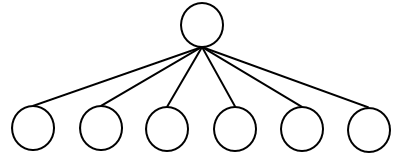
\includegraphics[scale = 0.4]{images/star-tree.png}
    \end{figure}

    The root in the network, receives the following sensor data $S_{1}(10), S_{2}(14), S_{3}(12), S_{4}(15), S_{5}(11),S_{6}(17)$ and has its own data $S_{0}(15)$. 

    The root node aggregates these seven data and creates an aggregated result as follows:
    \begin{equation}
      S = \sum_{i=0}^6 S_{i}
    \end{equation}
    Now, root has to send only one data to its parent instead of seven.
    \vfill
    \clearpage

  % \subsection*{Common Topologies}

  %     \begin{figure}
  %       \centering
  %       \begin{subfigure}
  %         \centering
  %         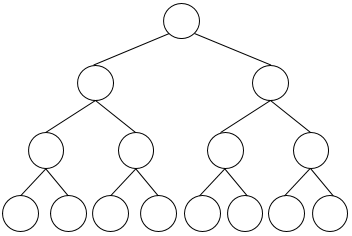
\includegraphics[width=.4\linewidth]{images/binary-tree.png}
  %         \caption{Binary Tree Network}
  %         \label{fig:binary-tree}
  %       \end{subfigure}

  %       \begin{subfigure}
  %         \centering
  %         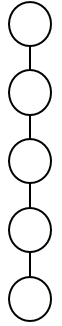
\includegraphics[scale=0.5]{images/palm-tree.png}
  %         \caption{Palm Tree Network}
  %         \label{fig:palm-tree}
  %       \end{subfigure}%
        
  %       \begin{subfigure}
  %         \centering
  %         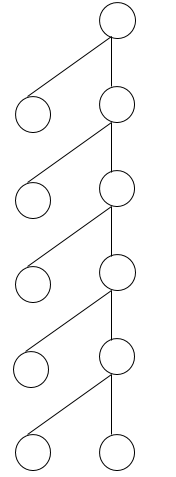
\includegraphics[scale=0.5]{images/pseudo-palm-tree.png}
  %         \caption{Palm Tree Network}
  %         \label{fig:palm-tree}
  %       \end{subfigure}%
  %     \end{figure}

  %     % \begin{figure}[h!]
  %     %   \begin{minipage}[b]{0.49\linewidth}
  %     %     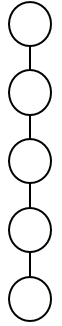
\includegraphics[scale=0.5]{images/palm-tree.png}
  %     %     \caption{Palm Tree} \label{fig:figure2}
  %     %   \end{minipage}

  %     %   \hspace{0.5cm}

  %     %   \begin{minipage}[b]{0.49\linewidth}
  %     %     \centering
  %     %     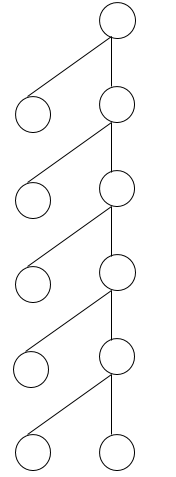
\includegraphics[scale=0.5]{images/pseudo-palm-tree.png}
  %     %     \caption{brain} \label{fig:figure2}
  %     %   \end{minipage}

  %     % \end{figure}

  %     \clearpage

  \subsection*{Lossy Data Compression}
    \vfill
    Lossy data compression schemes produces a compressed file from which only an \textbf{approximation} to the original information can be recovered. Much higher compression ratios are possible.

    Our aggregation protocol is \textbf{lossy data compression} as the base station receives an aggregated sensor data and can not recover the original sensor data.
    \vfill
    \clearpage

\section*{Secure Hierarchical In-network Data Aggregation}
    \vfill
    SHIA is a light weight protocol for providing data-integrity to in-network data aggregation scheme.
    
    It is designed for general networks with single or multiple adversaries.
    
    Our work enhances SHIA, by making it communication efficient, adds new security services to the protocol, achieves similar security goals with non-resilient aggregation functions and efficient ways of analyzing the protocol.
    \vfill
    \clearpage

    \subsection*{Network Assumptions}
      \vfill
      A multi hop network with a set $ S = \{S_{1},...,S_{n}\} $ of $n$ nodes where all sensor nodes are alive and reachable. 

      The network is organized in a \textbf{rooted tree topology}.

      The \textbf{trusted base station} resides outside of the network and the network and the network topology. 

      The base station can directly communicate with every node in the network using \textbf{authenticated broadcast}.

      All the wireless communications is \textbf{peer-to-peer} and we do not consider the \textbf{local wireless broadcast}.

      Each sensor node $I$ has a unique \textbf{ID} and shares a unique secret symmetric key $\sf{sk}_{I}$ with the base station.

      The sensor nodes are capable of doing \textbf{symmetric and asymmetric} key encryption and decryption.
      \vfill
      \clearpage

    \subsection*{Attacker Model}
      \vfill
      We consider a model with \textbf{polynomially bounded} adversary (polynomial in terms of the security parameter), which has a complete control over some of the sensor nodes in the network.
   
      We focus on \textbf{stealthy attacks}, where the goal of an adversary is to make the base station accept false aggregation  results, which are significantly different from the true results determined by the measured values, while not being detected by the base station.
      
      We do not consider \textbf{denial-of-service (DoS)} and various \textbf{passive attacks}.
      \vfill
      \clearpage

    \subsection*{SUM Aggregate Algorithm}
      \vfill
      Here, the aggregate function $f$\ is summation meaning that we want to compute $a_{1} + a_{2} + \dotsc + a_{n}$, where $a_{i}$\ is the sensor reading of the node $i$.
 
      The algorithm has the following three main phases.
      \begin{description}
        \item [Query Dissemination,] initiates the aggregation process.
        \item [Aggregate Commit,] initiates the commitment tree generation process.
        \item [Result Checking,] initiates the distributed, interactive verification process.
      \end{description}
      \vfill
      \clearpage

    \subsection*{Aggregation Tree}
      \vfill
      We require the prior constructed rooted aggregation tree.
      \begin{figure}[h!]
        \centering
        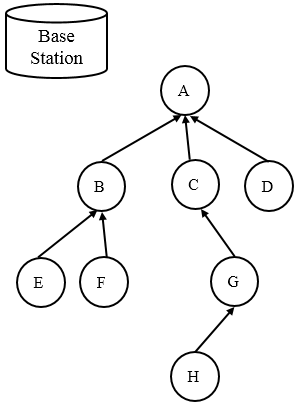
\includegraphics[scale=0.4]{images/aggregation-tree-1.png}
        \caption{Aggregation Tree.}
        \label{fig:Aggregation-tree-1}
      \end{figure}
      \vfill
      \clearpage

    \subsection*{Query Dissemination}
      \vfill
      The base station broadcasts the query request message with the query nonce $N$\ in the aggregation tree. 
    
      SHIA uses \textbf{hash chain} to generate new nonce for each query. 
      
      A hash chain is constructed by repeatedly evaluating a pre-image resistant hash function $h$\ on some initial random value, the final value (or ``anchor value'') is preloaded on the nodes in the network.
      
      The base station uses the pre-image of the last used value as the nonce for the next broadcast.
      
      \begin{figure}[h!]
        \centering
        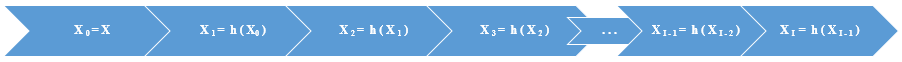
\includegraphics[scale=0.4]{images/hash-chain.png}
        \caption{Hash Chain.}
        \label{fig:hash-chain}
      \end{figure}

      For example, if the last known value of the hash chain is $h^i(X)$, then the next broadcast uses $h^{i-1}(X)$ as the nonce; $X$ is the initial random value.
      
      When a node receives a new nonce $N^{'}$, it verifies that $N^{'}$ is a precursor to the most recently received (and authenticated) nonce $N$ on the hash chain, i.e., $h^{i}(N^{'}) = N$ for some $i$ bounded by a fixed $k$ of number of hash applications.  
      \vfill
      % A hash chain prevents an adversary from predicting the query nonce for future queries as it has to reverse the hash chain computation to get an acceptable pre-image.
      \clearpage

% \section*{Our Protocol}
    
    \subsection*{Data Item}
      \vfill
      A commitment tree is a binary tree where each vertex has an associated data-item representing the data that is passed on to its parent.
      \begin{equation*}
        < id, count, value, commitment >
      \end{equation*}

      Each sensor node creates its own data-item. 
      For example, sensor node $A$ creates its data-item $A_{0}$.
      \begin{equation*}
        A_{0} =\ <A_{id}, 1, A_{value}, H(N||1||A_{value})>
      \end{equation*}
      where $A_{id}, A_{value}$ is the unique ID and sensor reading of the node $A$. 
      The count is $1$ as there is only vertex in the subtree rooted at $A$, $H$ is the collision resistant hash function, and $N$ is the query nonce.
      \vfill
    \clearpage

    \subsection*{Signing and Verification of the Data-item}
      \vfill
      Each sensor node sends the signature of its data-item signed by itself using its own secret key. 
      \begin{equation*}
          \textsf{S} = \textsf{Sign}_{\sk_{A}}(A_{0})
        \end{equation*}
        \begin{center}
          Table: Digital Certificate
      \end{center}
      \begin{table} 
        \tiny 
          \centering
          \begin{tabular}{ |l| }
              \hline
              Unique ID of the sensor node \\
              \hline
              Public key of the sensor node \\  
              \hline
              Certification Authority's name \\
              \hline
              Certification Authority's digital signature \\
              \hline
          \end{tabular}
        % \end{center}
      \end{table}

      \begin{equation*}
        \textsf{Verify}_{\pk_{A}}(A_{0},\textsf{S}) = 
        \begin{cases}
         \textbf{true}\ \mbox{with probability of 1} & \mbox{if}\ \textsf{S} = \textsf{Sign}_{\sk_{A}}(A_{0})\\
         \textbf{false}\ \mbox{with overwhelming probability} & \mbox{if}\ \textsf{S} \neq \textsf{Sign}_{\sk_{A}}(A_{0})
        \end{cases}
      \end{equation*}
      \vfill
      \clearpage

    \subsection*{Commitment Payload}
      \vfill
      A \textbf{commitment payload} is a set of data-items of the root vertices of the trees with their respective signatures in the outgoing commitment forest and an additional signature for the transmission.
    
      The \textbf{transmit payload} is the concatenation of all the data-items in the commitment payload.
      \vfill
      \clearpage

    \subsection*{Commitment Payload Example}
      \vfill
      \begin{figure}[h!]
        \centering
        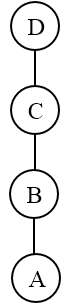
\includegraphics[scale = 0.5]{images/palm-aggregation-tree.png}
        \caption{Palm Shaped Aggregation Tree}
        \label{fig:Palm aggregation tree}
      \end{figure}

      \begin{equation*}
        A_{pay} =\ <A_{0}, \textsf{Sign}_{\sk_{A}}(A_{0}), \textsf{Sign}_{\sk_{A}}(A_{\tau}) >\ where\ A_{\tau} =\ < A_{0} > 
      \end{equation*}

      \begin{figure}[h!]
        \centering
        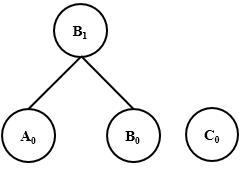
\includegraphics[scale = 0.5]{images/commitment-payload-of-C.png}
        \caption{Commitment Payload of Sensor Node $C$}
        \label{fig:Commitment payload of C}
      \end{figure}

      \begin{equation*}  
        \begin{array}{l}
          C_{pay} =\ <C_{0},\textsf{Sign}_{\sk_{C}}(C_{0}),B_{1},\textcolor{red}{\textsf{Sign}_{\sk_{B}}(B_{1})}, \textsf{Sign}_{\sk_{C}}(C_{\tau})>\ where\ C_{\tau} = <C_{0} || B_{1}>\\
          C_{0} =\ <C_{id}, 1, C_{value}, H(N||1||C_{value})>\\
          B_{1} =\ <B_{id}, 2, B_{1value}, H(N||2||B_{1value}||A_{0}||B_{0})>;\ B_{1value} =\ B_{value} + A_{value}
        \end{array}
      \end{equation*}
      \vfill
      \clearpage

    \subsection*{FSwRD vs FSwoRD}

      Forwarding Signatures With Resigning Data-Item (FSwRD)
      \begin{equation*}  
        \begin{array}{l}
          C_{pay} =\ <C_{0},\textsf{Sign}_{\sk_{C}}(C_{0}),B_{1},\textcolor{red}{\textsf{Sign}_{\sk_{C}}(B_{1})}, \textsf{Sign}_{\sk_{C}}(C_{\tau})>\ where\ C_{\tau} =\ <C_{0} || B_{1}>\\
        \end{array}
      \end{equation*}

      Forwarding Signatures Without Resigning Data-Item (FSwoRD)
      \begin{equation*}
          C_{pay} =\ <C_{0}, \textsf{Sign}_{\sk_{C}}(C_{0}), B_{1}, \textcolor{red}{\textsf{Sign}_{\sk_{B}}(B_{1})}, \textsf{Sign}_{\sk_{C}}(C_{\tau}) >\ where\ C_{\tau} =\ <C_{0} || B_{1}>\\
      \end{equation*}
      
      \vfill
      \clearpage

    \subsection*{Analogy for FSwRD vs FSwoRD}
      \begin{figure}[h!]
        \centering
        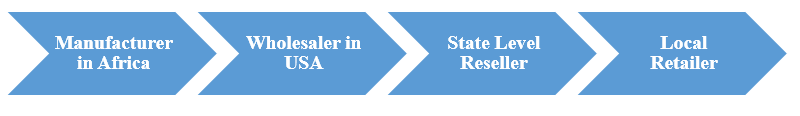
\includegraphics[scale=0.5]{images/diamond-supply-chain.png}
        \caption{Diamond Supply Chain.}
        \label{fig:diamond-supply-chain}
      \end{figure}
      \vfill
      \clearpage

    \subsection*{Security Benefits of Signatures}
      The signature allows the parent node to verify the \textbf{authenticity} of the sensor node and assures the \textbf{integrity} of the data-item.

      It allows the sender to have the proof for the sent data-item and the receiver to have the proof for the received data-item, providing the security service of \textbf{non-repudiation}.

      The digital signature depends on the message so the parent node can not reuse the signature for other messages in the future, protecting the network against the \textbf{replay attacks}.

      The signature of the transmit-payload is like the signature for the transmission, assuring none of the data-items in its payload have been left stranded.

      \vfill
      \clearpage

    % \subsection*{Query Dissemination}
    \vfill%   
    \clearpage

    \subsection*{Aggregate Commit}
      This phase creates the commitment tree for the given aggregation tree.
      % We describe the commitment tree generation process for an aggregation tree shown in Figure \ref{fig:Aggregation-tree-1}.
      % \begin{figure}[h!]
      %   \centering
      %   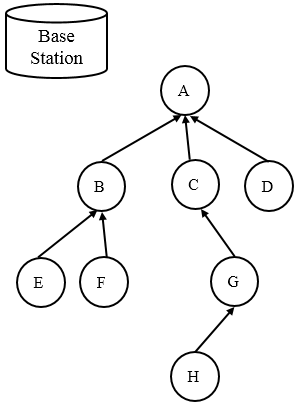
\includegraphics[scale=0.4]{images/aggregation-tree-1.png}
      %   \caption{Aggregation Tree.}
      %   \label{fig:Aggregation-tree-1}
      % \end{figure}

    \subsection*{Commitment Tree Generation}
    
      Leaf nodes in the aggregation tree construct and send their payload to their parents in the aggregation tree.  
      
      Each internal node in the aggregation tree constructs their leaf vertex.
  
      Internal node verifies all the received signatures then it merges all the data-items with same count value from its forest.

      It merges two data-items by creating a new data-item with count value incremented by one and whose value is the addition of value field of the previous two data-items. 

      For example, in Figure \ref{fig:Aggregation-tree-1}, the root $A$ receives payloads from each of its children.
        
      We describe the payload generation process for nodes $D,B,C$ and $A$ in order.
      \vfill
      \clearpage

    % \subsection*{Commitment Tree Generation Example}
    \vfill%   
    \clearpage

    \subsection*{Example Continue: D's Payload Generation}
      The node $D$ constructs its payload and sends $D_{pay}$ to its parent $A$.
      
      \begin{figure}[h!]
        \centering
        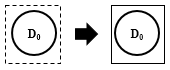
\includegraphics[scale = 0.5]{images/d-forest-payload.png}
        \caption{Transformation from $D$'s forest to its payload.
            Each dashed-line box shows forest and solid-line box shows payload of the respective sensor node.}
        \label{fig:d-forest-payload}
      \end{figure}
      \begin{equation*}
        \begin{array}{l}
          D_{pay} =\ <D_{0}, \textsf{Sign}_{\sk_{D}}(D_{0}), \textsf{Sign}_{\sk_{D}}(D_{\tau})>;\ where\ D_{\tau} =\ <D_{0}>\\
          \\
          D_{0} =\ <D_{id},1,D_{value},H(N||1||D_{value})>
        \end{array}
      \end{equation*}


      \vfill
      \clearpage

    \subsection*{Example Continue: B's Payload Generation}  
      The node $B$ constructs its payload from its forest which consists of payloads received from $E$ and $F$.

      Then node $B$ sends $B_{pay}$ to its parent $A$.
      \begin{figure}[h!]
        \centering
        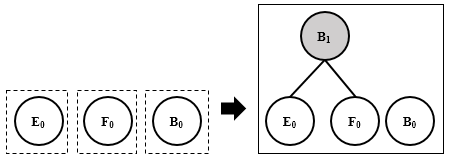
\includegraphics[scale = 0.5]{images/b-forest-payload.png}
        \caption{Transformation from $B$'s forest to its payload.}
        \label{fig:b-forest-payload}
      \end{figure}
      
      % \begin{equation*}
      %   \begin{array}{l}
      %   E_{pay} =\ <E_{0}, \textsf{Sign}_{\sk_{E}}(E_{0}), \textsf{Sign}_{\sk_{E}}(E_{\tau}) >\ where\ E_{\tau} =\ <E_{0}>\\
      %   F_{pay} =\ <F_{0}, \textsf{Sign}_{\sk_{F}}(F_{0}), \textsf{Sign}_{\sk_{F}}(F{\tau}) >\ where\ F_{\tau} =\ <F_{0}>
      %   \end{array}
      % \end{equation*}
      
      \begin{equation*}
        \begin{array}{l}
          B_{1} =\ < B_{id}, 2, B_{1value}, H(N||2||B_{1value}||E_{0}||F_{0})>;\ B_{1value} = E_{value} + F_{value}\\
          \\
          B_{pay} =\ < B_{0}, \textsf{Sign}_{\sk_{B}}(B_{0}), B_{1}, \textsf{Sign}_{\sk_{B}}(B_{1}), \textsf{Sign}_{\sk_{B}}(B_{\tau}) >\ where\ B_{\tau} =\ <B_{0} || B_{1}>\\
        \end{array}
        \label{eq:b-payload}
      \end{equation*}


      \vfill
      \clearpage
    
    \subsection*{Example Continue: C's Payload Generation}  
      The node $C$ constructs its payload from its forest which consists of payloads received from $G$.

      Then node $C$ sends $C_{pay}$ to its parent $A$.

      \begin{figure}[h!]
        \centering
        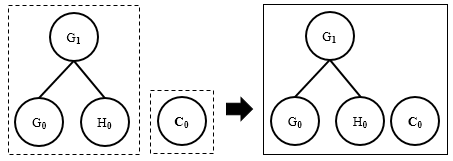
\includegraphics[scale = 0.5]{images/c-forest-payload.png}
        \caption{$C$'s forest aggregation creating its payload.}
        \label{fig:c-forest-payload}
      \end{figure}
      \begin{equation*}
        \begin{array}{l}
          G_{pay} =\ <G_{1},\textcolor{red}{\textsf{Sign}_{\sk_{G}}(G_{1})}, \textsf{Sign}_{\sk_{G}}(G_{\tau})>\ where\ G_{\tau} =\ <G_{0} || H_{0}>\\
        \end{array}
      \end{equation*}
      
      \begin{equation*}
        \begin{array}{l}
          C_{pay} =\ <C_{0},\textsf{Sign}_{\sk_{C}}(C_{0}),G_{1},\textcolor{red}{\textsf{Sign}_{\sk_{C}}(G_{1})}, \textsf{Sign}_{\sk_{C}}(C_{\tau})>\ where\ C_{\tau} =\ <C_{0} || G_{1}>\\
        \end{array}
        %\label{eq:c-payload}
      \end{equation*}

      \vfill
      \clearpage

    \subsection*{Example Continue: A's Payload Generation}  

      The root node of the aggregation tree $A$ receives the payloads from $B,C$ and $D$ respectively.
      
      \begin{figure}[h!]
        \centering
        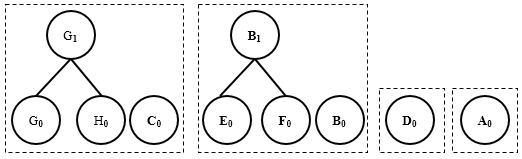
\includegraphics[scale = 0.5]{images/a-forest.png}
        \caption{$A$'s forest: $A$ receives three payloads from $C,B$ and $D$}
        \label{fig:a-forest}
      \end{figure}
      \vfill
      \clearpage

      \begin{figure}[h!]
        \centering
        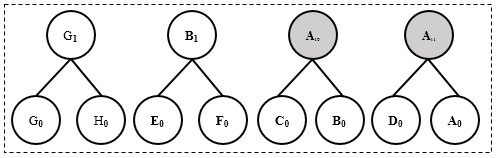
\includegraphics[scale = 0.5]{images/a-forest-first-merge.png}
        \caption{$A$'s forest: after first merge}
        \label{fig:a-forest-first-merge}
      \end{figure}
      \begin{equation*}
        \begin{array}{l}
          A_{10} =\ <A_{id},2,A_{10value},H(N||2||A_{10value}||B_{0}||C_{0})>;\ A_{10value} =\ B_{value} + C_{value}\\
          A_{11} =\ <A_{id},2,A_{11value},H(N||2||A_{11value}||D_{0}||A_{0})>;\ A_{11value} =\ D_{value} + A_{value}\\
        \end{array}     
      \end{equation*}

      \begin{figure}[h!]
        \centering
        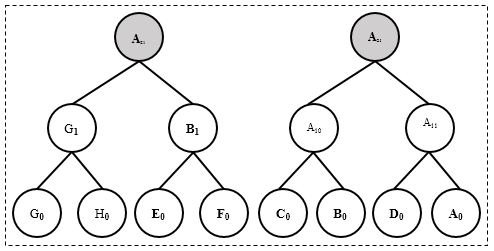
\includegraphics[scale = 0.5]{images/a-forest-second-merge.png}
        \caption{$A$'s forest: after second merge}
        \label{fig:a-forest-second-merge}
      \end{figure}

      \begin{equation*}
        \begin{array}{l}
          A_{20} =\ <A_{id},4,A_{20value},H(N||4||A_{20value}||G_{1}||B_{1})>;\ A_{20value} =\ G_{1value} + B_{1value}\\ 
          A_{21} =\ <A_{id},4,A_{21value},H(N||4||A_{21value}||A_{10}||A_{11})>;\ A_{21value} =\ A_{10value} + A_{11value}\\ 
        \end{array}
      \end{equation*}

      \begin{figure}[h!]
        \centering
        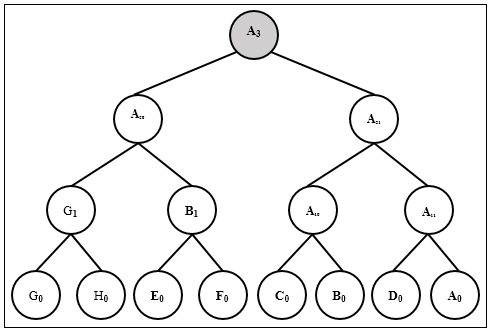
\includegraphics[scale = 0.5]{images/a-payload.png}
        \caption{$A$'s payload : $A$ sends $A_{3}$ to the base station.}
        \label{fig:a-payload}
      \end{figure}

      \begin{equation*}
        \begin{array}{l}
        A_{3} =\ <A_{id}, 8, A_{3value}, H(N||8||A_{3value}||A_{20}||A_{21})>;\ A_{3value} =\ A_{20value} + A_{21value}\\
        A_{pay} =\ <A_{3},\textsf{Sign}_{\sk_{A}}(A_{3}),\textsf{Sign}_{\sk_{A}}(A_{\tau})>\ where\ A_{\tau} =\ <A_{3}>
        \end{array}
      \end{equation*}
     \vfill
     \clearpage

  \section*{Result Checking}
    This phase requires that all the sensor nodes verify their individual contributions to the final aggregate value.

    If there is any inconsistency in the aggregation process then with the help of the base station, trace down the node responsible for inconsistency.

    It has the following major steps :
    \begin{description}
      \item [Dissemination of Final Payload by the Base Station]
      \item [Dissemination of Off-Path Values]
      \item [Verification of Inclusion]
      \item [Collection of Authentication Codes]
      \item [Verification of Authentication Codes]
      \item [Detecting An Adversary]
    \end{description}

    \vfill
    \clearpage

    \subsection*{Dissemination of Final Payload by the Base Station}

      The base station broadcasts all the data-items in the payload to entire network using \textbf{authenticated broadcast}.
        
      The base station receives only one data-item $A_{3}$ in the payload sent by $A$.
      
      The base station broadcasts $B_{pay}$ to entire network.

      \begin{equation*}
        \textsf{B}_{pay} =\ <A_{3}, \textsf{Sign}_{\sk_{\textsf{B}}}(A_{3}), \textsf{Sign}_{\sk_{\textsf{B}}}(\textsf{B}_{\tau})>\ where\ \textsf{B}_{\tau} =\ <A_{3}>.
      \end{equation*}
      \vfill
      \clearpage

      \subsection*{Dissemination of Off-Path Values}
        
        \begin{defn}
          The set of \textbf{off-path vertices} for a vertex $u$ in a tree is the set of all the siblings of each of the vertices on the path from $u$ to the root of the tree that $u$ is in (the path is inclusive of $u$).
        \end{defn}
        \begin{figure}[h!]
          \centering
          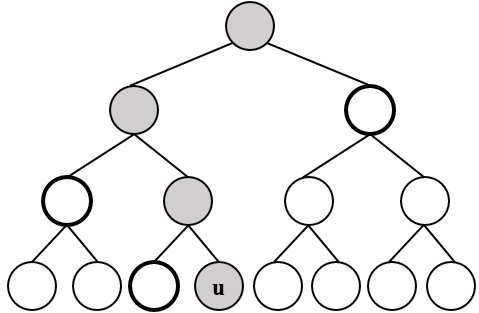
\includegraphics[scale = 0.4]{images/off-path.png}
          \caption{Off-path vertices of $u$ are highlighted in bold.}
          \label{fig:commitment-tree-example-2-shia}
        \end{figure}
        \vfill
        \clearpage

        In Figure \ref{fig:a-payload}, $A_{10}$ has two children $C_{0}$ and $B_{0}$.
        
        $A_{10}$ also receives $A_{11}$ and $A_{20}$ from its parent $A_{21}$.
        
        $A_{10}$ ( which is sensor node $A$ in aggregation tree ) sends the following off-path values to $C$ and $B$ respectively.
        
        % $A_{10}$ (which is sensor node $A$ in aggregation tree) sends the following off-path values to $C$ and $B$.
        
        % \begin{equation*}
        %   \begin{array}{l}
        %     <B_{0}, \textsf{Sign}_{\sk_{A}}(B_{0}),\textsf{Sign}_{\sk_{A}}(A_{\tau})>\ where\ A_{\tau} =\ <B_{0}>\\
        %     <C_{0}, \textsf{Sign}_{\sk_{A}}(C_{0}),\textsf{Sign}_{\sk_{A}}(A_{\tau})>\ where\ A_{\tau} =\ <C_{0}>.
        %   \end{array}
        % \end{equation*}
        
        \begin{equation*}
          \begin{array}{l}
            <B_{0}, \textcolor{red}{\textsf{Sign}_{\sk_{A}}(B_{0})},A_{11},\textsf{Sign}_{\sk_{A}}(A_{11}),A_{20},\textsf{Sign}_{\sk_{A}}(A_{20}),\textsf{Sign}_{\sk_{A}}(A_{\tau})>\\
              \\
              % \textcolor{white}{XXXXX}where\  A_{\tau} =\ <B_{0}||A_{11}||A_{20}>\\
            <C_{0}, \textcolor{red}{\textsf{Sign}_{\sk_{A}}(C_{0})},A_{11},\textsf{Sign}_{\sk_{A}}(A_{11}),A_{20},\textsf{Sign}_{\sk_{A}}(A_{20}),\textsf{Sign}_{\sk_{A}}(A_{\tau})>\\ 
              % \textcolor{white}{XXXXX}where\  A_{\tau} =\ <C_{0}||A_{11}||A_{20}>.
          \end{array}
        \end{equation*}
        \vfill
        \clearpage

      \subsection*{FSwoRD}
        \begin{equation*}
          \begin{array}{l}
            <B_{0}, \textcolor{red}{\textsf{Sign}_{\sk_{B}}(B_{0})},A_{11},\textsf{Sign}_{\sk_{A}}(A_{11}),A_{20},\textsf{Sign}_{\sk_{A}}(A_{20}),\textsf{Sign}_{\sk_{A}}(A_{\tau})>\\
              \\
              % \textcolor{white}{XXXXX}where\  A_{\tau} =\ <B_{0}||A_{11}||A_{20}>\\
            <C_{0}, \textcolor{red}{\textsf{Sign}_{\sk_{C}}(C_{0})},A_{11},\textsf{Sign}_{\sk_{A}}(A_{11}),A_{20},\textsf{Sign}_{\sk_{A}}(A_{20}),\textsf{Sign}_{\sk_{A}}(A_{\tau})>\\ 
              % \textcolor{white}{XXXXX}where\  A_{\tau} =\ <C_{0}||A_{11}||A_{20}>.
          \end{array}
        \end{equation*}

        In FSwRD, all the leaf vertices need to know only one certificate as they receive data-items signed by their parent vertex.

        In FSwoRD, all the leaf vertices might need to know $\log l$ certificates, where $l$ is the number of leaf-vertices in commitment tree.
        \vfill
        \clearpage

      \subsection*{Significance of Commitment Filed}

        The commitment filed provides data-integrity and helps us detecting any \textit{malicious activity} in the network. 
        The signatures infrastructure eventually we can detect an adversary. 

        If an internal vertex simply \textbf{forwards incorrect data-item} then the relevant leaf vertex will complain, as they will not be able to derive the data-item received using authenticated broadcast from the base station.
        
        If an internal vertex \textbf{changed the data-item} while creating commitment tree and sending the incorrect off-path values to compensate discrepancy. 
        \vfill
        \clearpage

      \subsection*{Malicious Activity}

        Suppose the vertices in the commitment tree have the data-items defined as follows :
        
        \begin{equation*}
          \begin{array}{l}
            A_{0} =\ <A_{id},1,10, H(N||1||10)>\\
            B_{0} =\ <B_{id},1,20, H(N||1||20)>\\
            C_{1} =\ <C_{id},2,30, H(N||2||30||A_{0}||B_{0})>
          \end{array}
        \end{equation*}

        \begin{figure}
          \centering
          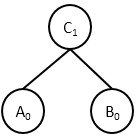
\includegraphics[scale=0.6]{images/commitment-tree-2.png}
          \label{fig:smallest-ct}
          \tiny{\caption{Smallest Possible Commitment Tree}}
        \end{figure}
        \vfill
        \clearpage

        Suppose $C$ changes $A_{0}$ and $B_{0}$ to $A'_{0}$ and $B'_{0}$.

        $C$ can send either $C'_{1}$ or $C''_{1}$ to the base station.
        
        To compensate for the discrepancy, $C$ constructs $B''_{0}$ and $A''_{0}$ off-path values trying to hide its malicious activity from the base station.

        \begin{equation*}
          \begin{array}{l}
            A'_{0} =\ <A_{id},1,100, H(N||1||10)>\\
            B'_{0} =\ <B_{id},1,200, H(N||1||20)>\\
            \\
            C'_{1} =\ <C_{id},2,300, H(N||2||300||\mathbf{A''_{0}}||\mathbf{B_{0}})>\ or \\ 
            C''_{1} =\ <C_{id},2,300, H(N||2||300||\mathbf{A_{0}}||\mathbf{B''_{0}})>\\
            \\
            B''_{0} = <B_{id},1,290,H(N||1||20)>\\
            A''_{0} = <A_{id},1,280,H(N||1||10)>
          \end{array}
        \end{equation*}
        \vfill
        \clearpage

        $A$ and $B$ receives either $C'_{1}$ or $C''_{1}$ from the base station based on what $C$ has sent to base station.

        $A$ and $B$ receives $B''_{0}$ and $A''_{0}$ from $C$ respectively.

        $A$ and $B$ derives the root data-item using the received off-path values, and it does not match with the received root data-item.

        \begin{equation*}
          \begin{array}{l}
            A\ \mbox{uses}\ (A_{0}, B''_{0})\ \mbox{and derives} <2,300,H(N||2||300||\mathbf{A_{0}}||\mathbf{B''_{0}})>\  = C''_{1} \neq C'_{1} \\
            B\ \mbox{uses}\ (A''_{0}, B_{0})\ \mbox{and derives} <2,300,H(N||2||300||\mathbf{A''_{0}}||\mathbf{B_{0}})>\  = C'_{1} \neq C''_{1}.
          \end{array}
        \end{equation*}

        The commitment field makes it nearly impossible for an adversary to tamper with the data-items while creating commitment tree and/or while distributing off-path values.
        \vfill
        \clearpage

\clearpage

\section*{\LaTeX{ } Workshop}

\vspace{.75in}

\end{slide}
\end{document}
Brian King

\vspace{.1in}

\verb1briking@iupui.edu1\\
\verb1http://et.engr.iupui.edu/~briking/latex/1

\clearpage

\subsection*{\LaTeX{}}

\mybul A  document typesetting system -- 

\mybul Open Source software 

\mystr available Windows, Unix/Linux, Mac,

\mybul high-quality: camera-ready output

\mybul can produce a number of different outputs PostScript, PDF, HTML, etc

\mybul there exists packages that support thesis, music, chemistry,....


\clearpage
\subsection*{Benefits of \LaTeX}

\mybul Excellent for producing thesis quality, journal
article, conference paper

\mybul can produce books and online content
(HTML, PDF)


\mybul Standard styles (such as IEEE) available

\mybul High quality results with little effort

\mybul trivial to modify article from one style to another (see experiment)



\clearpage


\subsection*{How does it work? What do you need?}

\mybul Authors write documents -- require editor 
%markup-language -- file will have a \verb1.tex1 extension\\
turn extensions on in your computer


\mybul Run a \LaTeX processor to produce a
device-independent file (dvi)  or run \verb1pdflatex1 to produce a \verb1pdf1
or run \verb1xelatex1  to produce \verb1pdf1  (when using images that are \verb1.eps1)

\mybul for a dvi file use a previewer like YAP to view the dvi file


\mybul Edit, Process, Preview cycle during
production

\mybul  \textcolor{red}{\bf what do we need? \ty{editor}....textpad, notepad, emacs, VI editor, crimson editor,texworks...}

\mybul to \verb1pdflatex1 use texworks or...\\
\myws \myws \mybul open \ty{command window}, change the directory to folder containing file  \\
\myws\myws \verb1cd C:\Documents and Settings\bk\Desktop\latex_work1\\
\myws\myws   execute the \verb1 pdflatex  file_name1 command
%
%\mybul run the previewer  \myws enter  \verb1yap file1 in command window

\clearpage

\section*{Where to get it}

Miktex
\url{http://miktex.org/}
\\


\noindent to download
\url{http://miktex.org/download}


download installer


run 

will download latex, ...\\

also texworks   a editor, latex builder, etc




\clearpage

\subsubsection*{What does ''tex'' look like? (from wikipedia)}

\begin{tiny}
\begin{verbatim}
\documentclass[12pt]{article}
\usepackage{amsmath}
\title{\LaTeX}
\date{}
\begin{document}
  \maketitle 
  \LaTeX{} is a document preparation system for the \TeX{} 
  typesetting program. It offers programmable desktop publishing 
  features and extensive facilities for automating most aspects of 
  typesetting and desktop publishing, including numbering and 
  cross-referencing, tables and figures, page layout, bibliographies, 
  and much more. \LaTeX{} was originally written in 1984 by Leslie 
  Lamport and has become the dominant method for using \TeX; few 
  people write in plain \TeX{} anymore. The current version is 
  \LaTeXe.
 
  % This is a comment, it is not shown in the final output.
   The following shows a little of the typesetting power of LaTeX
  \begin{align}
    E &= mc^2    \\                          
    m &= \frac{m_0}{\sqrt{1-\frac{v^2}{c^2}}}
  \end{align}
\end{document}
\end{verbatim}
\end{tiny}

\clearpage

%\begin{center}
\includegraphics[scale=0.5]{sw.pdf}
%\nolinebreak
%\hspace{.3in}
%\includegraphics[width=60mm,height =2in]{combiner.jpg}
%\end{center}



\clearpage



\LaTeX{} is designed to separate content from
presentation\\

The author should focus on the text and
structure\\

Layout, fonts and presentation determined by
style\\


%\clearpage


De facto standard for many disciplines in
academia\\

Also gaining acceptance in publishing houses
Computer Science, Engineering, Physics, Mathematics all
have very demanding typesetting
requirements\\

\LaTeX{} allows publishers to provide style file
and produce high-quality consistent results
for conferences, journals, etc.




\clearpage

Many commands are followed by arguments\\ %When commands are followed by arguments, the format is: 
\myws \verb1 \command{argument} 1

\begin{verbatim}
\section*{My first document} 
\url{http://www.silmaril.ie/downloads/} 
\end{verbatim}

%Another example of a command with an argument is \documentclass{article} this tells LaTeX to read your work as a document, and one formatted as an article. Articles don't have separate title pages, but chapters and books do, so if you want to have separate title pages from the actual text of the work, you would do \documentclass{chapter} or \documentclass{book}. 


\ty{Defining the Document}

\LaTeX{} needs the document to be defined in order to properly process the document. 
This is the first item defined in a LaTeX document and it's defined with the command 
\begin{verbatim}
\documentclass[options]{class}. 
\end{verbatim}


\clearpage

\ty{Document Classes}

article: for conference and other presentations, short reports, anything written that's relatively small 
and less formatted (around 1-20 pages, no chapter breaks) 

report: for longer works containing several chapters, small books, PhD dissertations, Master's theses book for real books 

seminar: for slides.
% FoilTeX is generally viewed as a better option for this, and with FoilHTML, slides can also be converted to HTML. 

\clearpage


\ty{\bf Document Class Options }

\textcolor{red}{\bf SKIP}

10pt, 11pt, 12pt: This sets the size of the main font in the document. If no option is specified, 10pt is assumed. 

letterpaper, legalpaper: This defines the paper size. The default size is letterpaper. a5paper, b5paper, executivepaper, and legalpaper can be specified. 

fleqn: This is used for papers with mathematical formulae. This typesets displayed formulae left-aligned instead of centred. leqno Places the numbering of formulae on the left hand side instead of the right. 

titlepage, notitlepage: This specifies whether a new page should be started after the document title or not. The article class does not start a new page by default, while report and book do. 

onecolumn, twocolumn: This tells LaTeX to typeset the document in one column or two columns and is used most often for specific typesetting needs. 

twoside, oneside: This specifies whether double or single sided output should be generated. The classes article and report are single sided and the book class is double sided by default. Note that this option concerns the style of the document only. The option twoside does not tell the printer you use that it should actually make a two-sided printout. 

landscape: This changes the layout of the document to print in landscape mode. 

openright, openany: This makes chapters begin either only on right hand pages or on the next page available. This does not work with the article class, as it does not know about chapters. The report class by default starts chapters on the next page available and the book class starts them on right hand pages. 

\clearpage

\ty{Page Styles}

\LaTeX{} supports three predefined header/footer combinations, which are often called page styles. The style parameter of the command defines which one to use. The command to call a page style is:

\begin{verbatim}
\pagestyle{style}\end{verbatim}


The predefined page styles are: 

plain: This prints the page numbers on the bottom of the page, in the middle of the footer. This is the default page style. 

headings: This prints the current chapter heading and the page number in the header on each page, while the footer remains empty. (This is the style used in this document) 

empty: This sets both the header and the footer to be empty. 


\clearpage
\subsubsection*{\LaTeX{} preamble}

\begin{verbatim}
\documentclass[12pt]{article} 
\usepackage{url,graphicx,amsmath}
\begin{document} 
\end{verbatim}

your text will lie between \verb1\begin{document}1
and \verb1\end{document}1
\\

for every \verb1\begin{..}1
there should be a \verb1\end{...}1

\clearpage

\begin{tiny}
\begin{verbatim}
\documentclass[12pt]{article} 
\usepackage{palatino,url} 
\begin{document} 
\section*{My first document} 
This is a short example of a \LaTeX\ document 
I wrote on \today. It shows a few simple features 
of automated typesetting, including 

\begin{itemize} 
\item setting the default font to 12pt; 
\item specifing `article' type formatting; 
\item using the palatino typeface; 
\item adding special formatting for URLs; 
\item formatting a deading in `section' style; 
\item using the \LaTeX\ logo; 
\item generating today's date; 
\item centering and italicizing; 
\item autonumbering the pages. 
\end{itemize} 

\subsection*{More information} 

This example was taken from `Formatting Information,' 
which you can download from \url{http://www.silmaril.ie/downloads/} 
and use as a teach-yourself guide. 

\clearpage

\begin{center} 
\itshape Have a nice day! 
\end{center} 

\end{document} 

\end{verbatim}
\end{tiny}





\clearpage

\begin{tiny}
%\begin{verbatim}
%\documentclass[12pt]{article} 
%\usepackage{palatino,url} 
%\begin{document} 
\section*{My first document} 
This is a short example of a \LaTeX\ document 
I wrote on \today. It shows a few simple features 
of automated typesetting, including 

\begin{itemize} 
\item setting the default font to 12pt; 
\item specifing `article' type formatting; 
\item using the palatino typeface; 
\item adding special formatting for URLs; 
\item formatting a deading in `section' style; 
\item using the \LaTeX\ logo; 
\item generating today's date; 
\item centering and italicizing; 
\item autonumbering the pages. 
\end{itemize} 

\subsection*{More information} 

This example was taken from `Formatting Information,' 
which you can download from \url{http://www.silmaril.ie/downloads/} 
and use as a teach-yourself guide. 

\begin{center} 
\itshape Have a nice day! 
\end{center} 

%\end{document} 

%\end{verbatim}
\end{tiny}





\clearpage



\subsection*{Symbols}

\mybul Extensive symbol libraries available 

%\clearpage

\subsection*{Graphics}
\mybul Import: photos, graphs, diagrams, charts, etc.

\mybul Generate: diagrams, figures, etc.

\mybul Formats: many common image formats
supported

\clearpage

\subsection*{Bibliography}

\textcolor{red}{\bf SKIP}

\mybul BibTeX is a textual database of references

\mybul Bibliographies are generated for each
document

\mybul Citation style determined by bib style

\mybul EndNote can export to BibTeX

\mybul Online citation databases provide BibTeX
references

%intro�latex.tex � An Introduction to LATEX � Gavin Baker � 7/11/2002 � 11:05 � p. 18/29

\clearpage
\subsection*{Transparencies}

\textcolor{red}{\bf SKIP}

\mybul This presentation was produced with \LaTeX{} %the
%prosper 
and seminar packages

\mybul Easily produce slides %to rival PowerPoint

\mybul Generate for online viewing or printing to
transparencies

\mybul Various styles available

\mybul Customize layout, fonts, colors, etc

\clearpage

\subsection*{Output}
\LaTeX{} can generate a variety of output formats

DVI: device independent (preview, print,
convert)

HTML: produce online books and articles

PostScript: for printing

PDF: online display, presentations,
exchange



%intro�latex.tex � An Introduction to LATEX � Gavin Baker � 7/11/2002 � 11:05 � p. 23/29


\clearpage

%\clearpage
\subsection*{Links}

\textcolor{red}{\bf To download \LaTeX for the PC/Windows}

\verb1http://miktex.org/1
\\



\textcolor{red}{\bf Purdue Thesis Class } \\
\myws \verb1https://engineering.purdue.edu/~mark/puthesis/1



\clearpage

\subsection*{Quick introduction}


%\mybul we will expand on this on Thursday


\mybul there are a number of reserved symbols

\mybul \verb1$1 \\
\myws\myws the \$ initiates \textcolor{red}{math mode}, the \$ terminates math mode\\
\myws\myws example 
\begin{verbatim}
my favorite function is 
$f(x) =\log x +\cos 2\theta +\frac{x-2}{2x+1}$
\end{verbatim}

output is\\
\myws my favorite function  is $f(x) =\log x +\cos 2\theta +\frac{x-2}{2x+1}$
\\


\mybul A paragraph is created by inserting a blank line (a single blank line  cause a new paragraph, there is no additional effect by having more than one blank line 

\mybul \% will comment out all content on the line to the right of \%

\mybul \verb1\\1 starts a new line, this has a difference between starting a paragraph

\mybul empty line starts a new paragraph

\mybul multiple empty lines are equivalent to one empty line, 

\clearpage

\myws 

\clearpage
\begin{tiny}
\begin{table}
\begin{tabular}{*8l}
\X\alpha        &\X\theta       &\X o           &\X\tau         \\
\X\beta         &\X\vartheta    &\X\pi          &\X\upsilon     \\
\X\gamma        &\X\gamma       &\X\varpi       &\X\phi         \\
\X\delta        &\X\kappa       &\X\rho         &\X\varphi      \\
\X\epsilon      &\X\lambda      &\X\varrho      &\X\chi         \\
\X\varepsilon   &\X\mu          &\X\sigma       &\X\psi         \\
\X\zeta         &\X\nu          &\X\varsigma    &\X\omega       \\
\X\eta          &\X\xi                                          \\
                                                                \\
\X\Gamma        &\X\Lambda      &\X\Sigma       &\X\Psi         \\
\X\Delta        &\X\Xi          &\X\Upsilon     &\X\Omega       \\
\X\Theta        &\X\Pi          &\X\Phi
\end{tabular}
\caption{Greek Letters}\label{greek}
\end{table}
\end{tiny}


%\clearpage
\clearpage

\begin{tiny}


\begin{table}
\begin{tabular}{*8l}
\X\pm           &\X\cap         &\X\diamond             &\X\oplus     \\
\X\mp           &\X\cup         &\X\bigtriangleup       &\X\ominus    \\
\X\times        &\X\uplus       &\X\bigtriangledown     &\X\otimes    \\
\X\div          &\X\sqcap       &\X\triangleleft        &\X\oslash    \\
\X\ast          &\X\sqcup       &\X\triangleright       &\X\odot      \\
\X\star         &\X\vee         &\X\lhd$^b$             &\X\bigcirc   \\
\X\circ         &\X\wedge       &\X\rhd$^b$             &\X\dagger    \\
\X\bullet       &\X\setminus    &\X\unlhd$^b$           &\X\ddagger   \\
\X\cdot         &\X\wr          &\X\unrhd$^b$           &\X\amalg     \\
\X+             &\X-
\end{tabular}

$^b$ Not predefined in a format based on {\tt basefont.tex}.
     Use one of the style options\\
     {\tt oldlfont}, {\tt newlfont}, {\tt amsfonts} or {\tt amssymb}.

\caption{Binary Operation Symbols}\label{bin}
\end{table}
\end{tiny}

\clearpage

\begin{tiny}


\begin{table}
\begin{tabular}{*8l}
\X\leq          &\X\geq         &\X\equiv       &\X\models      \\
\X\prec         &\X\succ        &\X\sim         &\X\perp        \\
\X\preceq       &\X\succeq      &\X\simeq       &\X\mid         \\
\X\ll           &\X\gg          &\X\asymp       &\X\parallel    \\
\X\subset       &\X\supset      &\X\approx      &\X\bowtie      \\
\X\subseteq     &\X\supseteq    &\X\cong        &\X\Join$^b$    \\
\X\sqsubset$^b$ &\X\sqsupset$^b$&\X\neq         &\X\smile       \\
\X\sqsubseteq   &\X\sqsupseteq  &\X\doteq       &\X\frown       \\
\X\in           &\X\ni          &\X\propto      &\X=            \\
\X\vdash        &\X\dashv       &\X<            &\X>            \\
\X:
\end{tabular}

$^b$ Not predefined in a format based on {\tt basefont.tex}.
     Use one of the style options\\
     {\tt oldlfont}, {\tt newlfont}, {\tt amsfonts} or {\tt amssymb}.

\caption{Relation Symbols}\label{rel}
\end{table}
\end{tiny}

\clearpage

\begin{tiny}

\begin{table}
\begin{tabular}{*{5}{lp{3.2em}}}
\X,     &\X;    &\X\colon       &\X\ldotp       &\X\cdotp
\end{tabular}
\caption{Punctuation Symbols}\label{punct}
\end{table}

\begin{table}
\begin{tabular}{*6l}
\X\leftarrow            &\X\longleftarrow       &\X\uparrow     \\
\X\Leftarrow            &\X\Longleftarrow       &\X\Uparrow     \\
\X\rightarrow           &\X\longrightarrow      &\X\downarrow   \\
\X\Rightarrow           &\X\Longrightarrow      &\X\Downarrow   \\
\X\leftrightarrow       &\X\longleftrightarrow  &\X\updownarrow \\
\X\Leftrightarrow       &\X\Longleftrightarrow  &\X\Updownarrow \\
\X\mapsto               &\X\longmapsto          &\X\nearrow     \\
\X\hookleftarrow        &\X\hookrightarrow      &\X\searrow     \\
\X\leftharpoonup        &\X\rightharpoonup      &\X\swarrow     \\
\X\leftharpoondown      &\X\rightharpoondown    &\X\nwarrow     \\
\X\rightleftharpoons    &\X\leadsto$^b$
\end{tabular}

$^b$ Not predefined in a format based on {\tt basefont.tex}.
     Use one of the style options\\
     {\tt oldlfont}, {\tt newlfont}, {\tt amsfonts} or {\tt amssymb}.

\caption{Arrow Symbols}
\end{table}
\end{tiny}

\clearpage

\begin{tiny}

\begin{table}
\begin{tabular}{*8l}
\X\ldots        &\X\cdots       &\X\vdots       &\X\ddots       \\
\X\aleph        &\X\prime       &\X\forall      &\X\infty       \\
\X\hbar         &\X\emptyset    &\X\exists      &\X\Box$^b$     \\
\X\imath        &\X\nabla       &\X\neg         &\X\Diamond$^b$ \\
\X\jmath        &\X\surd        &\X\flat        &\X\triangle    \\
\X\ell          &\X\top         &\X\natural     &\X\clubsuit    \\
\X\wp           &\X\bot         &\X\sharp       &\X\diamondsuit \\
\X\Re           &\X\|           &\X\backslash   &\X\heartsuit   \\
\X\Im           &\X\angle       &\X\partial     &\X\spadesuit   \\
\X\mho$^b$      &\X.            &\X|
\end{tabular}

$^b$ Not predefined in a format based on {\tt basefont.tex}.
     Use one of the style options\\
     {\tt oldlfont}, {\tt newlfont}, {\tt amsfonts} or {\tt amssymb}.

\caption{Miscellaneous Symbols}\label{ord}
\end{table}
\end{tiny}

\clearpage

\begin{tiny}

\begin{table}
\begin{tabular}{*6l}
\X\sum          &\X\bigcap      &\X\bigodot     \\
\X\prod         &\X\bigcup      &\X\bigotimes   \\
\X\coprod       &\X\bigsqcup    &\X\bigoplus    \\
\X\int          &\X\bigvee      &\X\biguplus    \\
\X\oint         &\X\bigwedge
\end{tabular}
\caption{Variable-sized  Symbols}\label{op}
\end{table}


\begin{table}
\begin{tabular}{*8l}
\Z\arccos &\Z\cos  &\Z\csc &\Z\exp &
           \Z\ker    &\Z\limsup &\Z\min &\Z\sinh \\
\Z\arcsin &\Z\cosh &\Z\deg &\Z\gcd &
           \Z\lg     &\Z\ln     &\Z\Pr  &\Z\sup  \\
\Z\arctan &\Z\cot  &\Z\det &\Z\hom &
           \Z\lim    &\Z\log    &\Z\sec &\Z\tan  \\
\Z\arg    &\Z\coth &\Z\dim &\Z\inf &
           \Z\liminf &\Z\max    &\Z\sin &\Z\tanh
\end{tabular}
\caption{Log-like Symbols}\label{log}
\end{table}
\end{tiny}

\clearpage

\begin{tiny}


\begin{table}
\begin{tabular}{*8l}
\X(             &\X)            &\X\uparrow     &\X\Uparrow     \\
\X[             &\X]            &\X\downarrow   &\X\Downarrow   \\
\X\{            &\X\}           &\X\updownarrow &\X\Updownarrow \\
\X\lfloor       &\X\rfloor      &\X\lceil       &\X\rceil       \\
\X\langle       &\X\rangle      &\X/            &\X\backslash   \\
\X|             &\X\|
\end{tabular}
\caption{Delimiters\label{dels}}
\end{table}

\begin{table}
\begin{tabular}{*8l}
\Y\rmoustache&  \Y\lmoustache&  \Y\rgroup&      \Y\lgroup\\[5pt]
\Y\arrowvert&   \Y\Arrowvert&   \Y\bracevert
\end{tabular}
\caption{Large Delimiters\label{ldels}}
\end{table}

\end{tiny}

\clearpage

\begin{tiny}

\begin{table}
\begin{tabular}{*{10}l}
\W\hat{a}     &\W\acute{a}  &\W\bar{a}    &\W\dot{a}    &\W\breve{a}\\
\W\check{a}   &\W\grave{a}  &\W\vec{a}    &\W\ddot{a}   &\W\tilde{a}\\
\end{tabular}
\caption{Math mode accents}\label{accent}
\end{table}

\begin{table}
\begin{tabular}{*4l}
\W\widetilde{abc}       &\W\widehat{abc}                        \\
\W\overleftarrow{abc}   &\W\overrightarrow{abc}                 \\
\W\overline{abc}        &\W\underline{abc}                      \\
\W\overbrace{abc}       &\W\underbrace{abc}                     \\[5pt]
\W\sqrt{abc}            &$\sqrt[n]{abc}$&\verb|\sqrt[n]{abc}|   \\
$f'$&\verb|f'|          &$\frac{abc}{xyz}$&\verb|\frac{abc}{xyz}|
\end{tabular}
\caption{Some other constructions}\label{other}
\end{table}

\end{tiny}


\end{slide}
\end{document}

\verb1winedt1

In the late 70�s Donald Knuth created TEX and
METAFONT to typeset his book
In the early 80�s Leslie Lamport created LATEX
to make TEX easier to use
The TEX system was frozen years ago
LATEX core at 2 is stable
LATEX extensions throughout 90�s and 00�s
LATEX 3 is under development

\end{slide}
\end{document}
%intro�latex.tex � An Introduction to LATEX � Gavin Baker � 7/11/2002 � 11:05 � p. 11/29

\clearpage

arpage


\clearpage
\mybul what is \Latex 
\mywbul whhat are the benefits of using \Latex
\mybul 

\clearpage


lonks



\clearpage
introduction


demonstration



\subsection*{Collaboration}
Split up large documents into chapters or
sections

Selectively process different sections

Multiple authors can work independently on
files

Integrate with CVS for revision control
%intro�latex.tex � An Introduction to LATEX � Gavin Baker � 7/11/2002 � 11:05 � p. 21/29

\clearpage


